\documentclass[../main.tex]{subfiles}

\begin{document}
    % Während der grösste Teil des Guidebooks sich mit der Software selber beschäftigt,
    % wird hier die physikalische/virtuelle Infrastruktur in welche die Software installiert und betrieben wird beschrieben.
    % Folgende Fragen sollten hier behandelt werden:
    %   •Ist eine klare Infrastruktur Architektur vorhanden?
    %   •Welche Hardware (virtuell oder physikalisch) wird dazu verwendet?
    %   •Ist Redundanz, Failoverund Disaster-Recovery vorgesehen?
    %   •Ist die Skalierung der Infrastruktur bekannt?
    %   •Wer ist zuständig für Support und Unterhalt der Infrastruktur?
    %   •Wer ist verantwortlich für die Ressourcen (ownership)?
    %   •etc.
    % Sehr oft enthält dieses Kapitel ein Infrastruktur/Netzwerk-Diagramm, welchesdie verschiedenen Hardware/Softwarekomponenten beschreibt und aufzeigt wie diese zusammenhängen.
    % Dieses Kapitel sollte in jedem Software-Guidebook enthalten sein.
    
    \section{Infrastructure Architecture}

    \par Das Spiel \gls{hexxle} läuft auf der Enigne Unity. Unity übernimmt das lokale Rendering, sowie die Ausführung von Scripts und Animationen. Der Vorteil von Unity ist, dass es erlaubt das Spiel sehr einfach auf verschieden Plattformen zur Verfügung zu stellen. Für das erste Release wird \gls{hexxle} aber nur auf Windows lauffähig sein. Es ist aber geplant, \gls{hexxle} in einem späteren Release auch für andere Plattformen wie MacOS oder auf Mobile wie Android/iOS zur Verfügung zu stellen.      

    \begin{figure}[H]
		\centering
		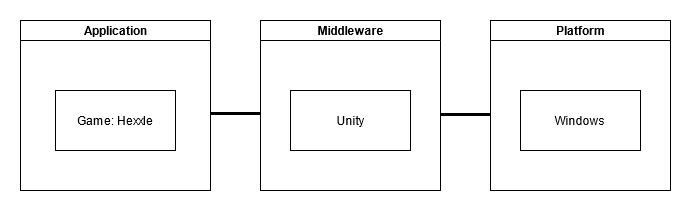
\includegraphics[angle=0, width=0.6\linewidth]{Architecture_Infrastructure.jpg}
	\end{figure}


\end{document}
